% !TEX root = ../../../main.tex
% 来源：中学数学实验教材·第三册（高中数学）
% 章节：二次函数 / 多项式函数的增减性
% 原始文件：5.tex，行 2276-2288
% 类型：tikz
% ---
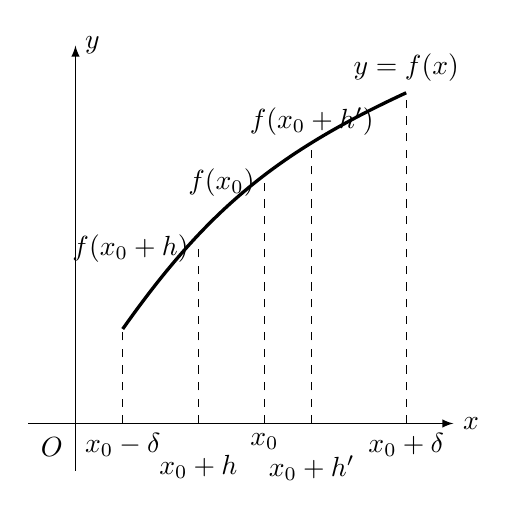
\begin{tikzpicture}[>=latex, scale=1.2]
    \draw[->] (-.5,0)--(4,0)node[right]{$x$};
    \draw[->] (0,-.5)--(0,4)node[right]{$y$};  
\draw [very thick](.5,1)to [bend right=-15](3.5,3.5)node[above]{$y=f(x)$};
\node at (-.25,-.25){$O$};
\draw[dashed] (.5,0)node[below]{$x_0-\delta$}--(.5,1);  
\draw[dashed] (3.5,0)node[below]{$x_0+\delta$}--(3.5,3.5);
\draw[dashed] (2,0)node[below]{$x_0$}--(2,2.55)node[left]{$f(x_0)$};

\draw[dashed] (1.3,0)node[below=8pt]{$x_0+h$}--(1.3,1.85)node[left]{$f(x_0+h)$};  
\draw[dashed] (2.5,0)node[below=8pt]{$x_0+h'$}--(2.5,2.95)node[above]{$f(x_0+h')$};

    \end{tikzpicture}
